\documentclass[11pt]{article}

%%%%%%%%%%%%%%Include Packages%%%%%%%%%%%%%%%%%%%%%%%%%%
\usepackage{xcolor}
\usepackage{mathtools}
\usepackage[a4paper, total={6in, 8in}, margin=1.25in]{geometry}
\usepackage{amsmath}
\usepackage{amssymb}
\usepackage{paralist}
\usepackage{rsfso}
\usepackage{amsthm}
\usepackage{wasysym}
\usepackage[inline]{enumitem}   
\usepackage{hyperref}
\usepackage{tocloft}
\usepackage{titlesec}
\usepackage{colortbl}
\usepackage{wrapfig}
\usepackage{pdfpages}
%%%%%%%%%%%%%%%%%%%%%%%%%%%%%%%%%%%%%%%%%%%%%%%%%%%%%%%%



\begin{document}
\begin{wrapfigure}[8]{r}{0.3\textwidth}
  \begin{center}
  \vspace{-15pt}
    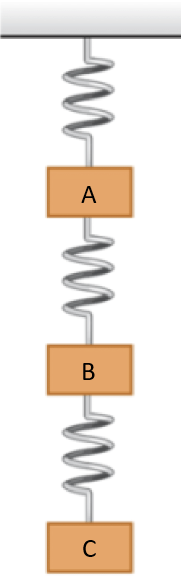
\includegraphics[scale=0.45]{springboxes}
  \end{center}
\end{wrapfigure}
\Large \noindent \textbf{Physics 1A Discussion (Week 5)}\\
\normalsize
Department of Physics and Astronomy, UCLA\\
\noindent\rule{8cm}{0.4pt}\\

\noindent \textbf{Problem 1:} Please solve the problem symbolically. Consider three identical boxes of mass $m$ hang by identical massless springs as shown. The springs have spring constant $k$, and each has equilibrium length $L_0$ (the length of it with no stretching or compressing). \\

\noindent(a) Draw the free-body diagram for the boxes.\\

\noindent (b) Find the total length of the springs.


\vfill

\noindent \textbf{Hint}: \color{gray}
For part (b), solve the problem by obtaining a set of three equations with three unknowns from the three free-body diagrams of the boxes. 
\color{black}

\newpage
\noindent \textbf{Problem 2:} Consider lifting crates that are $30$\,kg each from the ground to the bed of a truck that is $0.9$\,m off of the ground. You are lifting $6$ crates per minute.\\

\noindent (a) What is the power needed in this process? First compute it in the SI unit (W), then convert it into horsepower (hp).\\

\noindent (b) Suppose that you manage to continue lifting the crates for an entire hour, how many food calories do you burn?


\vfill

\noindent\textbf{Hint}: \color{gray}
Each horsepower (hp) is $746$ watts (W). \\
\color{black}
\textbf{Hint}: \color{gray}
Each calorie (cal) is $4.184$ Joules (J). \\
\color{black}


\newpage
\textbf{Boxes hang by springs}: When boxes are hang by the springs, the springs will all stretch. We solve this problem using the free-body diagrams of the boxes.\\
\begin{center}
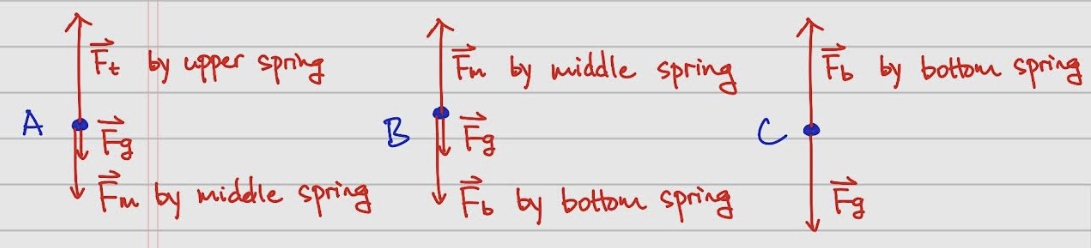
\includegraphics[scale=0.5]{fbdBoxes}
\end{center}
For box $A$ at equilibrium (zero acceleration, all forces get balanced), we have in the vertical direction
\begin{align*}
F_{t} - F_{m} - m g = 0\,,
\end{align*}
for $F_t$ is the force by the upper spring, and $F_m$ is the force by the middle spring. For box $B$, in the vertical direction,
\begin{align*}
F_m - F_b - m g = 0\,,
\end{align*}
where $F_b$ is the force due to the bottom spring. For box $C$, in the vertical direction, 
\begin{align*}
F_b - m g = 0\,.
\end{align*}
Here we have a system of three equations with three unknowns $F_t,\ F_m,\ F_b$. Solving this system we find
\begin{align*}
F_b = mg\,,\qquad
F_m = 2mg\,,\qquad
F_t = 3mg\,.
\end{align*}
Now applying $F = k\,\Delta x = k(L - L_0)$ to each of the springs (notice here $\Delta x$ is the displacement from equilibrium, that means the total length of the spring is $L$ instead of $\Delta x = L- L_0$ when the spring is stretched is providing a spring force $F$), for instance, for the bottom spring,
\begin{align*}
F_b = mg = k(L_b-L_0)\,,
\end{align*}
we obtain $L_b = mg/k + L_0$ to be the length of the bottom spring. Similarly we find $L_m = 2mg/k + L_0$ for the middle spring and $L_t = 3mg/k + L_0$ for the top spring. Thus the total length of the springs is 
\begin{align*}
L_b + L_m + L_t = \frac{6mg}{k} + 3L_0\,.
\end{align*}
\newpage
\textbf{Lifting crates}: First we compute the work done each time we lift one crate, 
\begin{align*}
W = \vec{F}\cdot \vec{d} = (30 \cdot 9.8)\,\text{N} \times 0.9 \,\text{m}= 264.6\,\text{J}\,.
\end{align*}
We are lifting $6$ boxes per minute, that is $0.1$ box per second. We do this conversion because the SI unit for power (watts) is measured in Joules per second. That is, it takes $(264.6\cdot 0.1)$\,J per second to lift the boxes. The power is thus
\begin{align*}
P = 26.46\,\text{W}\,.
\end{align*}
Converting this to horsepower, 
\begin{align*}
P = \frac{26.46}{746}\, \text{hp} = 3.547\times 10^{-2}\,\text{hp}\,.
\end{align*}
Continue doing this for an hour ($3600$ seconds), the amount of work it takes is  
\begin{align*}
W = P t = (26.46\,\text{W}) \times (3600 \,\text{s}) = 95259 \,\text{J}\,. 
\end{align*}
Convert this to calories, 
\begin{align*}
W = \frac{95259}{4.184}\,\text{cal} = 22766\,\text{cal}\,.
\end{align*}
We want our final answer in food calories (Cal), so 
\begin{align*}
W = \frac{22766}{1000}\,\text{Cal} = 22.77 \,\text{Cal}\,.
\end{align*}



\end{document}


